\section{Técnicas y herramientas útiles para el procesamiento del habla}

En la presente sección veremos algunas técnicas y herramientas necesarias para procesar y obtener información de las señales de habla.

\subsection{Transformada de Fourier de tiempo corto}
\label{sec:stft}

\subsubsection{Definición}

Las señales de habla son señales del tipo no-estacionarias, es decir sus características cambian en función del tiempo. Esto dificulta analizarlas desde la representación de Fourier \cite{spoken_language_processing,speech_enhancement_theory_and_practice}.

Resulta conveniente definir una transformada de Fourier variante en el tiempo. Dada una señal discreta $x[m]$ y una función ventana $w[m]$, la transformada de Fourier de tiempo corto (STFT por sus siglas en inglés) se define como:

\begin{equation*}
	STFT\{x[n]\}_{(n, \omega)} = X_{(n, \omega)} = \sum_{m=-\infty}^{\infty} w[n-m]x[m]e^{-j \omega m}
\end{equation*}

La función $w[m]$ tiene como responsabilidad determinar qué porción de la señal $x[m]$ se está analizando para un determinado tiempo n. Generalmente las funciones ventana poseen un valor nulo para todo $m$ salvo en $L$ puntos, es decir

\begin{equation*}
	w[m] = 
	\begin{cases}
		0 & \text{si $0 > m > L - 1$} \\
		\text{otro} & \text{si $0 <= m <= L - 1$}
	\end{cases}
\end{equation*}

La STFT es una función de dos variables, el tiempo n y la frecuencia $\omega$. Dado un $n$ determinado, la STFT se la puede pensar como la transformada de Fourier de la señal $w[n-m] x[m]$. Por lo tanto la función $X(n,\omega)$ como función de $\omega$, tiene las mismas propiedades que la transformada de Fourier \cite{oppenheim_schafer}.

En la figura \ref{fig:ch2_stft_explained}-a podemos ver la función $x[m]$ y la función $w[n-m]$ para un $n$ determinado. En \ref{fig:ch2_stft_explained}-b podemos ver el resultado de multiplicar ambas funciones $x[m]w[n-m]$ y en \ref{fig:ch2_stft_explained}-c vemos la transformada de Fourier de $x[m]w[n-m]$.

\begin{figure}
	\centering
	\centerline{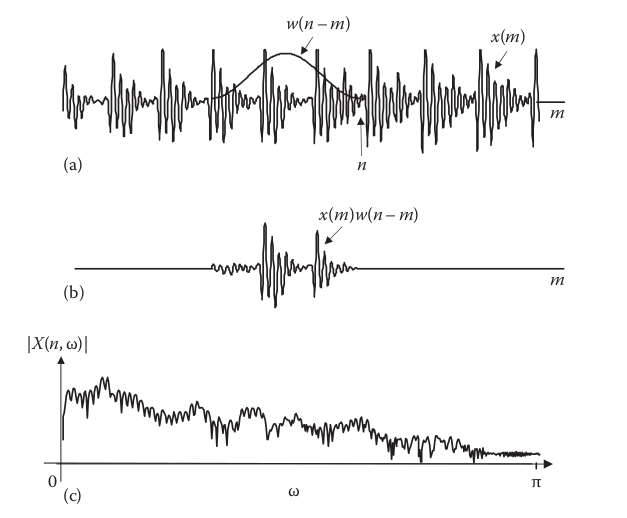
\includegraphics[scale=0.7]{images/ch2/stft_explained.png}}
	\caption{La STFT como la transformada de Fourier de la señal $w[n-m] x[m]$. Imagen tomada de \cite{speech_enhancement_theory_and_practice}.}
	\label{fig:ch2_stft_explained}
\end{figure}

Para la existencia de la STFT de $x[m]$ basta que la función $w[n-m]x[m]$ sea absolutamente sumable \cite{oppenheim_schafer} lo cual en general es cierto debido a la finita duración de $w[n-m]$.

La STFT permitirá hacer un procesamiento de las señales de habla en el dominio de la frecuencia. Sin embargo, una vez finalizado el análisis, será necesario volver al dominio del tiempo con lo que se necesitará la transformación inversa.

La secuencia $x[m]$ puede ser recuperada exactamente utilizando la ecuación de inversión de la transformada de Fourier:

\begin{equation*}
	w[n-m] x[m] = \frac{1}{2 \pi} \int_{- \pi}^{\pi} X(n, \omega) e^{j \omega m}
\end{equation*}

Haciendo $m=n$ y suponiendo $\omega(0) \neq 0$, tenemos que:

\begin{equation*}
	x[n] = \frac{1}{2 \pi \omega(0)} \int_{- \pi}^{\pi} X(n, \omega) e^{j \omega m}
\end{equation*}

Esta inversión es conceptual, en la práctica se trabaja en forma discreta y se recurre a métodos alternativos que veremos en las próximas secciones.

\subsubsection{Muestreo en tiempo y frecuencia}
\label{sec:muestreo_en_tiempo_y_frecuencia}

Dado que el procesamiento de las señales de habla se realiza de forma digital, es necesario contar con la versión discreta de la STFT. A partir de la definición de la DFT \cite{oppenheim_schafer}, se obtiene la versión discreta de la STFT por medio de muestrear la frecuencia en $N$ puntos separados uniformemente en $\omega_k = \frac{2 \pi k}{N}$ con $k = 0, 1, ..., N-1$. Por lo tanto la versión discreta de la STFT queda definida como:

\begin{equation*}
	STFT\{x[n]\}_{(n, \omega_k)} = X_{(n, \omega_k)} = \sum_{m=-\infty}^{\infty} x[m]w[n-m]e^{-j \omega_k m}
\end{equation*}

El proceso de ventanear la señal se podría repetir para cada $n$, es decir obtener la DFT de las secuencias: $w[0-m] x[m], w[1-m] x[m], w[2-m] x[m], ...$ para todo $n$. Esto resulta poco útil debido a que requiere mucho procesamiento y además se estaría obteniendo información redundante en el dominio de la frecuencia. 

Las DFTs obtenidas moviéndonos de a un $n$ a la vez, serían distintas, pero la información espectral sería prácticamente la misma. Para evitar este procesamiento ineficiente se suele tomar una ventana cada R muestras de la señal $x[m]$, es decir se realiza un muestreo en tiempo. 

La STFT muestreada en el tiempo queda definida como:

\begin{equation*}
	X_{(nR, \omega_k)} = \sum_{m=-\infty}^{\infty} x[m]w[nR-m]e^{-j \omega_k m}
\end{equation*}

Entonces, habrá tanto un muestreo en el dominio de la frecuencia como un muestreo en el dominio del tiempo, los cuales deben realizarse de manera tal que sea posible recuperar exactamente la señal $x[m]$.

De la DFT recordamos que para que no haya \emph{aliasing} en el dominio del tiempo se requiere que la variable de la frecuencia $\omega$ sea muestreada al menos $N$ veces para secuencias de largo $N$ \cite{oppenheim_schafer}. Dado que en nuestro caso las funciones $w[n-m] x[m]$ tienen largo $L$, tendremos a la primer restricción que es $N \geq L$.

Respecto de la elección del parámetro $R$, tendremos que si $R>L$, habrá ciertas muestras en el dominio del tiempo que se omitirán. Esto nos lleva a la segundo restricción que es $R \leq L$.

Las restricciones precedentes, nos llevan a la condición $R \leq L \leq N$ que de cumplirse permitirá recuperar la señal original $x[m]$. Estas restricciones son condiciones necesarias pero no suficientes. Dependiendo del tipo de método de reconstrucción que se utilice surgirán nuevas restricciones a cumplir. 

A continuación veremos el método de reconstrucción \emph{Overlapp-And-Add}, el cual tiene la ventaja de ser estable numéricamente \cite{oppenheim_schafer}, lo cual resulta esencial en aplicaciones de reducción de ruido.

\subsubsection{El método de reconstrucción Overlapp-And-Add}
\label{sec:overlapp_and_and}

El presente método de reconstrucción se basa en la siguiente ecuación \cite{jae_sung_oppenheim}:

\begin{equation*}
	\hat{x}[m] = \frac{R}{W(0)} \sum_{n=-\infty}^{\infty} \left[ \frac{1}{N} \sum_{k=0}^{N-1} X[mR, \omega_k] e^{j \omega_k n} \right]
\end{equation*}

\noindent donde:

\begin{equation*}
	W(0) = \sum_{m=-\infty}^{\infty} \omega[m]
\end{equation*}

El término entre corchetes no es más que la iDFT de las funciones $w[nR-m] x[m]$. Por lo tanto:

\begin{align*}
	\hat{x}[m] &= \frac{R}{W(0)} \sum_{n=-\infty}^{\infty} w[nR-m] x[m] \\
	&= x(m) \frac{R}{W(0)} \sum_{n=-\infty}^{\infty} w[nR-m]
\end{align*}

Entonces, para qué $\hat{x}[m] = x[m]$ se requiere que:

\begin{equation*}
	\sum_{n=-\infty}^{\infty} w[nR-m] = \frac{W(0)}{R} = C
\end{equation*}

Esta es la restricción que impone el método \emph{Overlapp-And-Add} en la función ventana $\omega[m]$, la cual se reduce a que al sumar todas las ventanas, se obtenga la constante $C$. 

Es posible trabajar esta ecuación para encontrar otras formas de expresar la restricción. Definimos la función  $\tilde{w}[m]$ como:

\begin{equation*}
	\tilde{w}[m] = \sum_{n=-\infty}^{\infty} w[nR-m]
\end{equation*}

Esta función es periódica con periodo R, con lo que se la puede escribir como la iDFT de $W[\omega_k]$ con $k = 0, 1, ..., R-1$:

\begin{equation*}
	\tilde{w}[m] = \frac{1}{R} \sum_{k=0}^{R-1} W[\omega_{k}] e^{j \omega_{k} m}
\end{equation*}

Si se cumpliese que $W[\omega_{k}]$ fuera 0 para $k = 1, 2, ..., R-1$, entonces se verificaría la condición original:

\begin{equation*}
	\tilde{w}[m] = \sum_{n=-\infty}^{\infty} w[nR-m] = \frac{W[0]}{R}
\end{equation*}

Entonces, la condición equivalente del método \emph{Overlapp-And-Add} es que la DFT de la función ventana tenga ceros para $k = 1, 2, ..., R-1$.

Existen diversos tipos de funciones ventana, cada una con sus propiedades. Para el análisis de señales por medio de la STFT se requiere tener bajos niveles de fuga espectral \cite{speech_enhancement_theory_and_practice}, lo que lleva al uso de funciones ventanas como la ventana de Hann o su variante, la ventana de Hamming \cite{oppenheim_schafer}.

La función ventana de Hann tiene sus ceros en las frecuencias $4 k \pi/M$ con $M = L - 1$ \cite{oppenheim_schafer}. Si estos ceros se alinearan con los requeridos por el método, la condición de reconstrucción sin pérdidas estaría verificada. Por lo tanto tenemos que:

\begin{equation*}
	\frac{2k\pi}{R} = \frac{4 k \pi}{M}
\end{equation*}

es decir, si elegimos $R$ tal que $R = M/2$, podremos reconstruir $x[m]$ sin pérdida de información.

\subsubsection{Espectrograma}
\label{sec:espectrograma}

La STFT es una función compleja. Una forma útil de analizar y de obtener información de las señales de habla es por medio del espectrograma que no es más que el módulo elevado al cuadrado de la STFT $|X_{(n, w)}^2|$. 

Usualmente el espectrograma es un gráfico en escala de colores o en escala de grises, donde a tonos más oscuros se tiene mayor energía para el tiempo y la frecuencia dados por los ejes \emph{x} e \emph{y} respectivamente. En la figura \ref{fig:ch2_spectrogram} podemos ver un ejemplo de una señal de habla junto a su espectrograma.

\begin{figure}[H]
	\centering
	\centerline{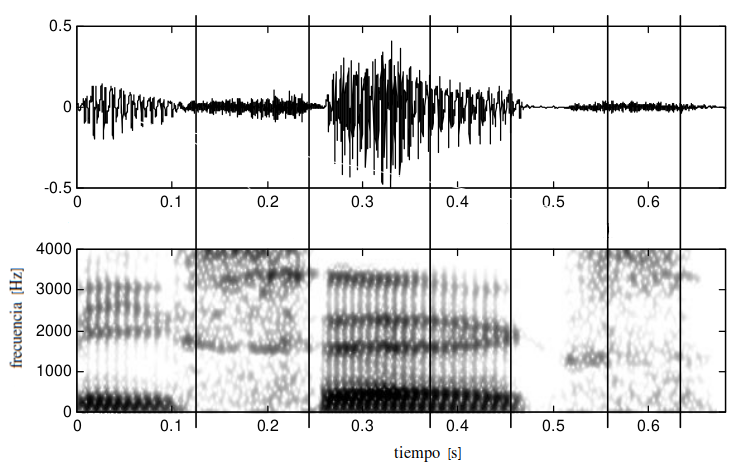
\includegraphics[scale=0.6]{images/ch2/spectrogram.png}}
	\caption{Señal de habla junto a su espectrograma. Imagen obtenida de \cite{spoken_language_processing}.}
	\label{fig:ch2_spectrogram}
\end{figure}

La STFT permite captar como cambian las características espectrales de una señal en función del tiempo. A medida que aumenta la velocidad con la que cambian las características de una señal, más corta se tendrá que hacer la ventana utilizada en la STFT. Sin embargo, a medida que la ventana se hace más corta, se pierde resolución en frecuencia. Esto se debe a que en general el ancho del lóbulo principal de una función ventana es inversamente proporcional al largo de ella y éste es el que principalmente determina la resolución en frecuencia.  Por ejemplo para la ventana de Hann y la de Hamming, el ancho del lóbulo principal es $8 \pi/L - 1$ \cite{oppenheim_schafer} 

Cuando se analizan señales de habla usando la STFT, y en particular usando un espectrograma, es posible notar diferentes características de la señal de habla dependiendo del tamaño de ventana utilizado. En la figura \ref{fig:ch2_wideband_narrowband} podemos ver en (a) un espectrograma con una ventana de $\SI{24}{ms}$ y en (b) un espectrograma con una ventana de $\SI{8}{ms}$. 

\begin{figure}[H]
	\centering
	\centerline{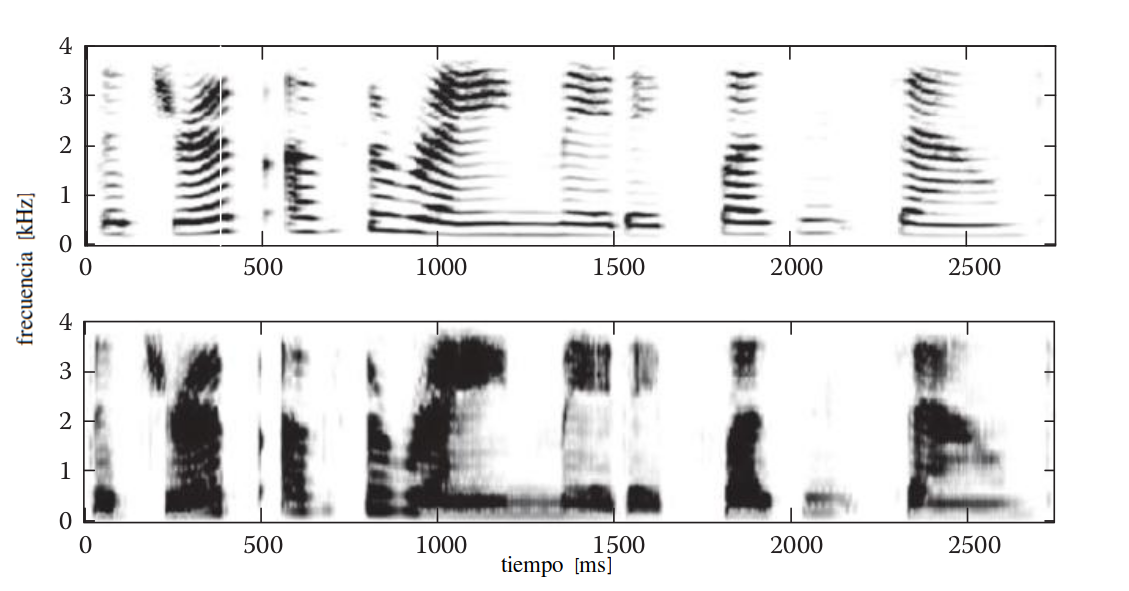
\includegraphics[scale=0.4]{images/ch2/wideband_narrowband.png}}
	\caption{Espectrograma de banda angosta y banda ancha. Imagen obtenida de \cite{speech_enhancement_theory_and_practice}.}
	\label{fig:ch2_wideband_narrowband}
\end{figure}

Los espectrogramas con ventanas de largos mayores a los $\SI{20}{ms}$ se llaman de banda angosta y se caracterizan por tener buena resolución en frecuencia. Estos espectrogramas permiten, por ejemplo, resolver las frecuencias de resonancia y sus armónicas, generadas por el tracto vocal en sonidos vocálicos \cite{spoken_language_processing}. Esto se puede ver en la figura \ref{fig:ch2_wideband_narrowband} (a) donde las armonices aparecen como líneas horizontales.

Los espectrogramas con ventanas de largo menores a los $\SI{10}{ms}$ se llaman de banda ancha y se caracterizan por tener buena resolución en el dominio del tiempo. Esto permite, por ejemplo, poder detectar sonidos de corta duración como las consonantes oclusivas \cite{spoken_language_processing}. Sin embargo, este tipo de espectrogramas oculta las armónicas como podemos ver en la figura \ref{fig:ch2_wideband_narrowband} (b).

En lo que concierne a la reducción de ruido en señales de habla, en general se busca poder reconocer los distintos fonemas contenidos en las señales de habla, lo que lleva a preferir ventanas de corto tiempo \cite{speech_enhancement_theory_and_practice}. Con ventanas cortas, tendremos una fina resolución en tiempo y resignaremos resolución en frecuencia.

\subsection{Sobre la importancia de la fase en las señales de habla} \label{sec:sobre_la_importancia_de_la_fase_en_las_señales_de_habla}

Usualmente los sistemas de supresión de ruido en señales de habla se basan en la estimación del espectrograma de la señal de habla, utilizando información presente en el espectrograma de la señal de habla ruidosa. Es decir, se estima únicamente la magnitud y no así la fase. En estos casos, la señal estimada se construye utilizando la magnitud estimada y la fase de la señal de habla ruidosa.

Dada la señal de habla ruidosa $x[n]$, su respectivo espectrograma $|X_{(n, w)}^2|$, su fase $\angle X_{(n, w)}$ y el espectrograma estimado de la señal de habla obtenida a la salida del filtro $|\hat{Y}_{(n, w)}^2|$, tenemos que:

\begin{equation*}
	\hat{Y}_{(n, w)} = |\hat{Y}_{(n, w)}| e^{i\angle X_{(n, w)}}
\end{equation*}

Esta suposición sobre la escasa importancia de la fase se basa en trabajos como el de Ohm sobre la ley de fase acústica \cite{ohm_s_law_of_acoustics}, en el cual se establece que la percepción de un tono de un sonido es una función de las amplitudes de las armónicas y no de la relación de fase entre ellas. 

Otros trabajos como \cite{the_unimportance_of_phase_in_speech_enhancement} realizaron estudios objetivos donde mezclaron magnitudes y fases a diferentes relaciones de señal a ruido (SNR por sus siglas en ingles), esto les permitió obtener una SNR equivalente la cual en la mayoría de los casos estaba dominada por la SNR de la magnitud.

Entonces, a la hora de diseñar un sistema para mejorar el nivel de ruido de una señal se debe prestar mayor atención a mejorar la SNR de la magnitud y no así la de la fase.


Si bien algunos estudios recientes como \cite{phase_importance_in_speech_processing_applications}, resaltan la importancia de contar con estimadores de calidad de la fase, el presente trabajo se concentrará únicamente en la estimación de la magnitud.


\subsection{Restricciones de tiempo y procesamiento}
\label{sec:time_restrictions}

Como vimos en la sección \ref{sec:objetivos}, el presente trabajo se limita al estudio del filtrado de ruido en señales de habla para aplicaciones de videoconferencias. A la hora de desarrollar sistemas de filtrado de ruido, el objetivo final del sistema pondrá restricciones en su diseño. Un sistema de filtrado pensado para aplicaciones de videoconferencias debe ser un sistema causal y de tiempo real.

Que sea causal implica que las estimaciones realizadas por el sistema se realizarán únicamente basadas en información pasada. Que sea de tiempo real implica que el tiempo de procesamiento del sistema debe ser tal que no supere la latencia máxima aconsejable para sistemas de comunicación virtual.

Los sistemas de comunicación virtual emulan una comunicación cara-a-cara. Cuando se utiliza un filtro de ruido las etapas son:

\begin{itemize}
	\item Se recibe la señal de habla de un participante
	\item Se filtran los ruidos indeseables
	\item Se envía la señal filtrada a los demás integrantes.
\end{itemize}

El tiempo total desde que se emite la señal de habla hasta que llega a los demás, no debe superar ciertos umbrales. Según la recomendación de la Unión Internacional de Telecomunicaciones \cite{itu_t_recommendation_g_114}, los participantes de una reunión virtual comenzarán a notar el retraso a partir de los $\SI{100}{ms}$ y la conversación dejará de ser fluida aproximadamente a partir de los $\SI{250}{ms}$.